\documentclass[a4paper]{article}

\usepackage[T1]{fontenc}
\usepackage[utf8]{inputenc}
\usepackage[italian]{babel}
\usepackage[a4paper]{geometry}
\usepackage[hidelinks]{hyperref}
\usepackage{eurosym}
\usepackage{caption, subcaption}
\usepackage{tikz, circuitikz}
\usepackage{pgf-umlcd, pgf-umlsd}

\renewcommand{\umltextcolor}{black}
\renewcommand{\umldrawcolor}{black}
\renewcommand{\umlfillcolor}{white}

\setlength{\parskip}{1.2ex}
\setlength{\parindent}{0em}
\clubpenalty = 100
\widowpenalty = 100

\title{CHIP-8 STM32}
\date{\today}
\author{Federico Bruzzone, Lorenzo Ferrante, Andrea Longoni \\
\footnotesize \texttt{\{federico.bruzzone, lorenzo.ferrante1, andrea.longoni3\}@studenti.unimi.it} \\ }

\begin{document}
\maketitle

\section{Introduzione}

% TODO: includere una foto dell'emulatore finito e funzionante

CHIP-8 è un linguaggio di programmazione creato a metà degli anni '70
da Joseph Weisbecker per semplificare lo sviluppo di videogiochi per
microcomputer a 8 bit. I programmi CHIP-8 vengono interpretati da una
macchina virtuale che è stata estesa parecchie volte nel corso degli
anni, tra le versioni più adottate citiamo S-CHIP e la più recente
XO-CHIP.

La semplicità dell'interprete in aggiunta alla sua lunga storia e
popolarità hanno fatto sì che emulatori e programmi CHIP-8 vengano
realizzati ancora oggi.
Nel corso degli anni molti videogiochi storici sono stati riscritti
in CHIP-8 tra cui Pong, Space Invaders e Tetris.

Lo scopo del progetto è quello di costruire un emulatore CHIP-8 e
S-CHIP in grado di funzionare su un microcontrollore STM32.

In questo documento ci riferiremo alla macchina virtuale che
interpreta programmi CHIP-8 con "interprete". Mentre utilizzeremo
"emulatore" per indicare l'interprete assieme ad una sua
implementazione (o "port"), ovvero un programma che gestisce
l'audio, il video, l'input da tastiera e interagisce con l'API della
macchina virtuale.

% TODO: migliorare lo scopo del progetto e accennare alle periferiche

\section{Hardware}

% TODO

\subsection{Schema di collegamento}

% TODO

\begin{figure}
\begin{center}
    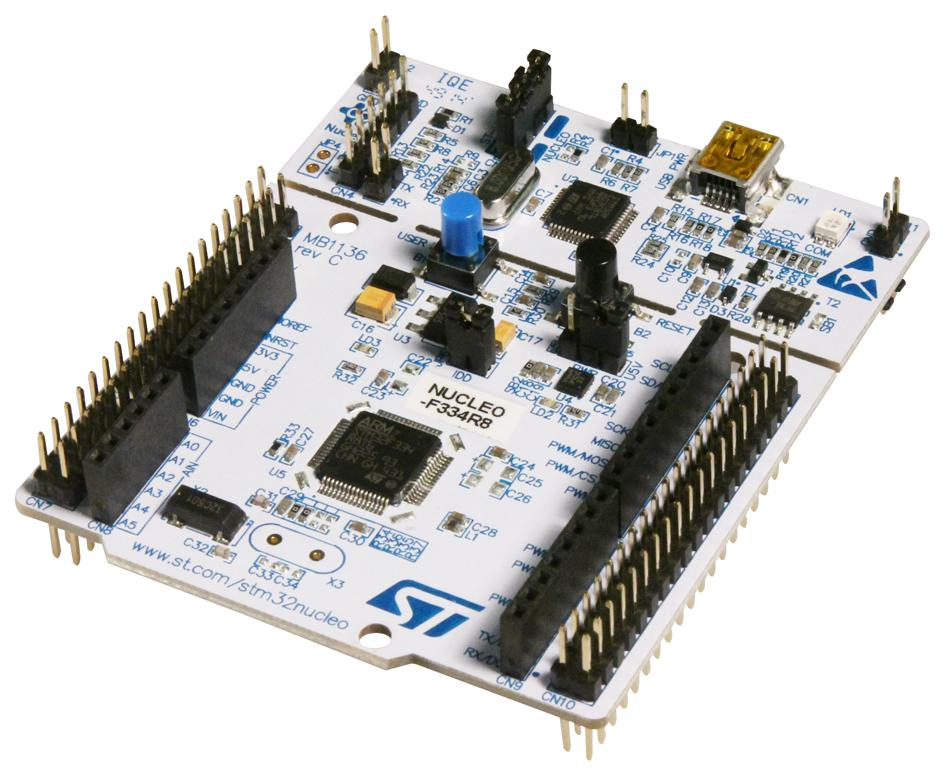
\includegraphics[scale=0.20]{figures/stm32f334.jpg}
\end{center}
\caption{Il microcontrollore \texttt{STM32F334R8T6}.}
\label{fig:stm32f334}
\end{figure}

\begin{figure}[h]
    \begin{subfigure}[b]{0.45\textwidth}
        \begin{center}
            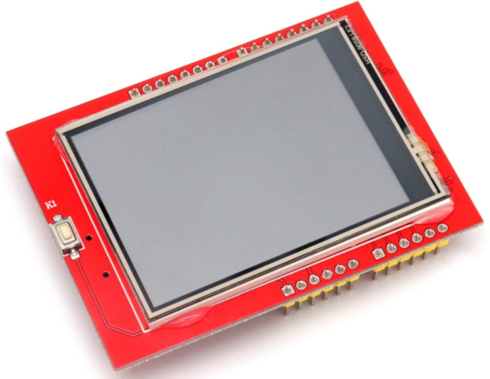
\includegraphics[scale=0.4]{figures/ili9341.png}
        \end{center}
        \caption{Lo schermo ILI9341.}
        \label{fig:ili9341}
    \end{subfigure}
    \hfill
    \begin{subfigure}[b]{0.45\textwidth}
        \begin{center}
            \begin{tikzpicture}[x=0.015cm, y=0.015cm, scale=0.75, transform shape]
                \draw   (120, 90) -- (320,90) -- (320,480) -- (120,480) -- cycle ;

\draw  [fill={rgb, 255:red, 255; green, 255; blue, 255 }  ,fill opacity=1 ]  (90,100)  --  (200,100) -- (200,130) --  (90,130) -- cycle;
\draw  [fill={rgb, 255:red, 255; green, 255; blue, 255 }  ,fill opacity=1 ]  (90,130)  --  (200,130) -- (200,160) --  (90,160) -- cycle;
\draw  [fill={rgb, 255:red, 255; green, 255; blue, 255 }  ,fill opacity=1 ]  (90,160)  --  (200,160) -- (200,190) --  (90,190) -- cycle;
\draw  [fill={rgb, 255:red, 255; green, 255; blue, 255 }  ,fill opacity=1 ]  (90,190)  --  (200,190) -- (200,220) --  (90,220) -- cycle;
\draw  [fill={rgb, 255:red, 255; green, 255; blue, 255 }  ,fill opacity=1 ]  (90,220)  --  (200,220) -- (200,250) --  (90,250) -- cycle;
\draw  [fill={rgb, 255:red, 255; green, 255; blue, 255 }  ,fill opacity=1 ]  (90,250)  --  (200,250) -- (200,280) --  (90,280) -- cycle;
\draw  [fill={rgb, 255:red, 255; green, 255; blue, 255 }  ,fill opacity=1 ]  (90,280)  --  (200,280) -- (200,310) --  (90,310) -- cycle;
\draw  [fill={rgb, 255:red, 255; green, 255; blue, 255 }  ,fill opacity=1 ]  (90,310)  --  (200,310) -- (200,340) --  (90,340) -- cycle;
\draw  [fill={rgb, 255:red, 255; green, 255; blue, 255 }  ,fill opacity=1 ]  (90,340)  --  (200,340) -- (200,370) --  (90,370) -- cycle;
\draw  [fill={rgb, 255:red, 255; green, 255; blue, 255 }  ,fill opacity=1 ]  (90,370)  --  (200,370) -- (200,400) --  (90,400) -- cycle;
\draw  [fill={rgb, 255:red, 255; green, 255; blue, 255 }  ,fill opacity=1 ]  (90,400)  --  (200,400) -- (200,430) --  (90,430) -- cycle;
\draw  [fill={rgb, 255:red, 255; green, 255; blue, 255 }  ,fill opacity=1 ]  (90,430)  --  (200,430) -- (200,460) --  (90,460) -- cycle;

\draw  [fill={rgb, 255:red, 255; green, 255; blue, 255 }  ,fill opacity=1 ] (250,100)  --  (380,100) -- (380,130) --  (250,130) -- cycle;
\draw  [fill={rgb, 255:red, 255; green, 255; blue, 255 }  ,fill opacity=1 ] (250,130)  --  (380,130) -- (380,160) --  (250,160) -- cycle;
\draw  [fill={rgb, 255:red, 255; green, 255; blue, 255 }  ,fill opacity=1 ] (250,160)  --  (380,160) -- (380,190) --  (250,190) -- cycle;
\draw  [fill={rgb, 255:red, 255; green, 255; blue, 255 }  ,fill opacity=1 ] (250,190)  --  (380,190) -- (380,220) --  (250,220) -- cycle;
\draw  [fill={rgb, 255:red, 255; green, 255; blue, 255 }  ,fill opacity=1 ] (250,220)  --  (380,220) -- (380,250) --  (250,250) -- cycle;
\draw  [fill={rgb, 255:red, 255; green, 255; blue, 255 }  ,fill opacity=1 ] (250,250)  --  (380,250) -- (380,280) --  (250,280) -- cycle;
\draw  [fill={rgb, 255:red, 255; green, 255; blue, 255 }  ,fill opacity=1 ] (250,280)  --  (380,280) -- (380,310) --  (250,310) -- cycle;
\draw  [fill={rgb, 255:red, 255; green, 255; blue, 255 }  ,fill opacity=1 ] (250,310)  --  (380,310) -- (380,340) --  (250,340) -- cycle;
\draw  [fill={rgb, 255:red, 255; green, 255; blue, 255 }  ,fill opacity=1 ] (250,340)  --  (380,340) -- (380,370) --  (250,370) -- cycle;


\draw (90,460) node [anchor=north west][inner sep=0.75pt]   [align=left] {$\displaystyle SD\_SCK$};
\draw (90,430) node [anchor=north west][inner sep=0.75pt]   [align=left] {$\displaystyle SD\_DO$};
\draw (90,400) node [anchor=north west][inner sep=0.75pt]   [align=left] {$\displaystyle SD\_DI$};
\draw (90,370) node [anchor=north west][inner sep=0.75pt]   [align=left] {$\displaystyle SD\_SS$};
\draw (90,340) node [anchor=north west][inner sep=0.75pt]   [align=left] {$\displaystyle LCD\_D1$};
\draw (90,310) node [anchor=north west][inner sep=0.75pt]   [align=left] {$\displaystyle LCD\_D0$};
\draw (90,280) node [anchor=north west][inner sep=0.75pt]   [align=left] {$\displaystyle LCD\_D7$};
\draw (90,250) node [anchor=north west][inner sep=0.75pt]   [align=left] {$\displaystyle LCD\_D6$};
\draw (90,220) node [anchor=north west][inner sep=0.75pt]   [align=left] {$\displaystyle LCD\_D4$};
\draw (90,190) node [anchor=north west][inner sep=0.75pt]   [align=left] {$\displaystyle LCD\_D5$};
\draw (90,160) node [anchor=north west][inner sep=0.75pt]   [align=left] {$\displaystyle LCD\_D3$};
\draw (90,130) node [anchor=north west][inner sep=0.75pt]   [align=left] {$\displaystyle LCD\_D2$};

\draw (250,370) node [anchor=north west][inner sep=0.75pt]   [align=left] {$\displaystyle 3.3V$};
\draw (250,340) node [anchor=north west][inner sep=0.75pt]   [align=left] {$\displaystyle 5V$};
\draw (250,310) node [anchor=north west][inner sep=0.75pt]   [align=left] {$\displaystyle GND$};
\draw (250,280) node [anchor=north west][inner sep=0.75pt]   [align=left] {$\displaystyle LCD\_RD$};
\draw (250,250) node [anchor=north west][inner sep=0.75pt]   [align=left] {$\displaystyle LCD\_WR$};
\draw (250,220) node [anchor=north west][inner sep=0.75pt]   [align=left] {$\displaystyle LCD\_RS$};
\draw (250,190) node [anchor=north west][inner sep=0.75pt]   [align=left] {$\displaystyle LCD\_CS$};
\draw (250,160) node [anchor=north west][inner sep=0.75pt]   [align=left] {$\displaystyle LCD\_RST$};
\draw (250,130) node [anchor=north west][inner sep=0.75pt]   [align=left] {$\displaystyle F\_CS$};

            \end{tikzpicture}
        \end{center}
        \caption{Pinout dello schermo \texttt{ILI9341}.}
        \label{fig:pinout_ili}
    \end{subfigure}
\end{figure}

\subsection{Materiali e costi} % ALT: Componenti e costi / Componenti utilizzati e relativi costi

\begin{center}
    \begin{table}[ht]
        \centering
        \begin{tabular}{|llll|l|}
            \hline
            \multicolumn{1}{|l|}{\textbf{Descrizione}}          & \multicolumn{1}{l|}{\textbf{Modello}}       & \multicolumn{1}{l|}{\textbf{Costo unitario}} & \textbf{Unità} & \textbf{Costo} \\ \hline
            \multicolumn{1}{|l|}{Microcontrollore}       & \multicolumn{1}{l|}{STM32 F334R8T6}         & \multicolumn{1}{l|}{14.99}                   & 1               & 14.99          \\ \hline
            \multicolumn{1}{|l|}{Schermo}                & \multicolumn{1}{l|}{ILI9341 2.4"}           & \multicolumn{1}{l|}{6.50}                    & 1               & 6.50           \\ \hline
            \multicolumn{1}{|l|}{Tastierino}          & \multicolumn{1}{l|}{Matrix keypad 4$\times$4} & \multicolumn{1}{l|}{3.99}                    & 1               & 3.99           \\ \hline
            \multicolumn{1}{|l|}{Beeper}                 & \multicolumn{1}{l|}{}                       & \multicolumn{1}{l|}{0.99}                    & 1               & 0.99           \\ \hline
            \multicolumn{1}{|l|}{Breadboard e cablaggio} & \multicolumn{1}{l|}{}                       & \multicolumn{1}{l|}{4.99}                    & 1               & 4.99           \\ \hline
            \multicolumn{4}{|r|}{\textbf{Totale}}                                                      & 31.50\euro    \\ \hline
        \end{tabular}
        \caption{
            Materiali utilizzati per la costruzione del progetto. I costi indicati provengono da negozi online come Amazon e eBay.
        }
    \end{table}
\end{center}

\section{Software}

Il nostro software si divide in due componenti principali:
l'interprete CHIP-8 e l'infrastruttura necessaria per "portarlo"
su un microcontrollore STM32, ovvero l'interfaccia con lo schermo
e i gestori per la scheda microSD, per il keypad e per il beeper.

\subsection{Interprete CHIP-8}

Abbiamo deciso di scrivere l'interprete da zero e per farlo è
stato necessario consultare le specifiche (de facto standard)
che definiscono il comportamento di un interprete
CHIP-8 \cite{cowgod:chip8} e S-CHIP \cite{cowgod:schip}.

L'interprete è scritto in C99, non ha I/O ed è freestanding
\cite{n1256:conformance}, ovvero non dipende dalla libreria
standard del C. Tutto questo è mirato a rendere l'interprete
altamente portabile.

Per rimuovere la dipendenza dalla libreria standard del C è stato
necessario includere alcune funzioni direttamente da libgcc, trovare
un modo alternativo per implementare le asserzioni e includere una
funzione ad hoc per la generazione di numeri casuali.

% TODO: aggiungere breve spiegazione della macchina virtuale

Per testare più comodamente l'interprete abbiamo sviluppato
un semplice emulatore su desktop utilizzando SDL2
\cite{libsdl:about}, una libreria scritta in C che consente di
gestire audio, video e input da tastiera.
In seguito l'interprete è stato sottoposto ad un'apposita
test suite \cite{github:chip8-test-suite} che mira a verificare
il comportamento corretto di ciascun opcode.

\subsubsection{Timing}

% TODO: spiegare meglio cosa si intende col timing e
% introdurre il problema legato ai timer vs frequenza dell'emu

Uno dei problemi principali durante lo sviluppo di un emulatore è
la gestione del timing.

In particolare abbiamo voluto disaccoppiare la frequenza
dell'emulatore (variabile e regolabile dal giocatore) dalla
frequenza del delay timer e del sound timer (costante a 60 Hz).

La frequenza dell'emulatore equivale al numero di istruzioni che
esegue ogni secondo.

Abbiamo sperimentato con due approcci diversi, nel primo il ritardo
del game loop è variabile e dipende dalla frequenza
dell'emulatore selezionata dal giocatore e ogni ciclo di emulazione
gestisce esattamente un'istruzione.
Mentre i timer vengono decrementati ogni n-esima iterazione del game
loop, dove n = EMU\_FREQ / 60.

Ad esempio, se EMU\_FREQ = 540, i timer vengono
decrementati ogni 9º ciclo (540 / 60 = 9).

Nel secondo approccio il ritardo del game loop è costante
a 16.666 ms per ottenere un frame rate di 60fps. In questo approccio,
ogni ciclo di emulazione gestisce un numero variabile di istruzioni.
Ad esempio, se EMU\_FREQ = 540, ogni ciclo di emulazione gestisce
9 istruzioni.

Dopo un attenta riflessione abbiamo deciso di impiegare il secondo
approccio. Il principale svantaggio del primo approccio è che chiama
una funzione simil-sleep per un periodo molto breve dopo ogni
istruzione, se EMU\_FREQ = 540, il ritardo di una sleep sarebbe
di circa 1.85 ms. Purtroppo questo tipo di funzione non offre questo
genere di precisione.

Per questo motivo abbiamo deciso di disaccoppiare la frequenza dei
timer (costante a 60 Hz) dalla frequenza dell'emulatore (variabile e
regolabile dal giocatore) utilizzando il secondo approccio.

Il ritardo del game loop è costante a 16.666 ms (per ottenere
un frame rate di 60 fps), mentre il numero di istruzioni eseguite
in ogni ciclo di emulazione è variabile.

Ciò consente di decrementare i timer dopo ogni ciclo di emulazione
a un tasso costante di 60 Hz.

Abbiamo considerato anche eventuali problematiche che sarebbero
potute sorgere con il secondo approccio. In particolare abbiamo
considerato il fatto che anche se non tutte le istruzioni richiedono
lo stesso tempo per essere eseguite, anche la più lenta richiede
una quantità trascurabile di tempo. Ciò significa che possiamo
comportarci come se tutte le istruzioni richiedessero il medesimo
tempo.

% TODO: non tutte le DRW vengono renderizzate

\subsubsection{Ottimizzazioni}

\begin{figure}
    \begin{center}
        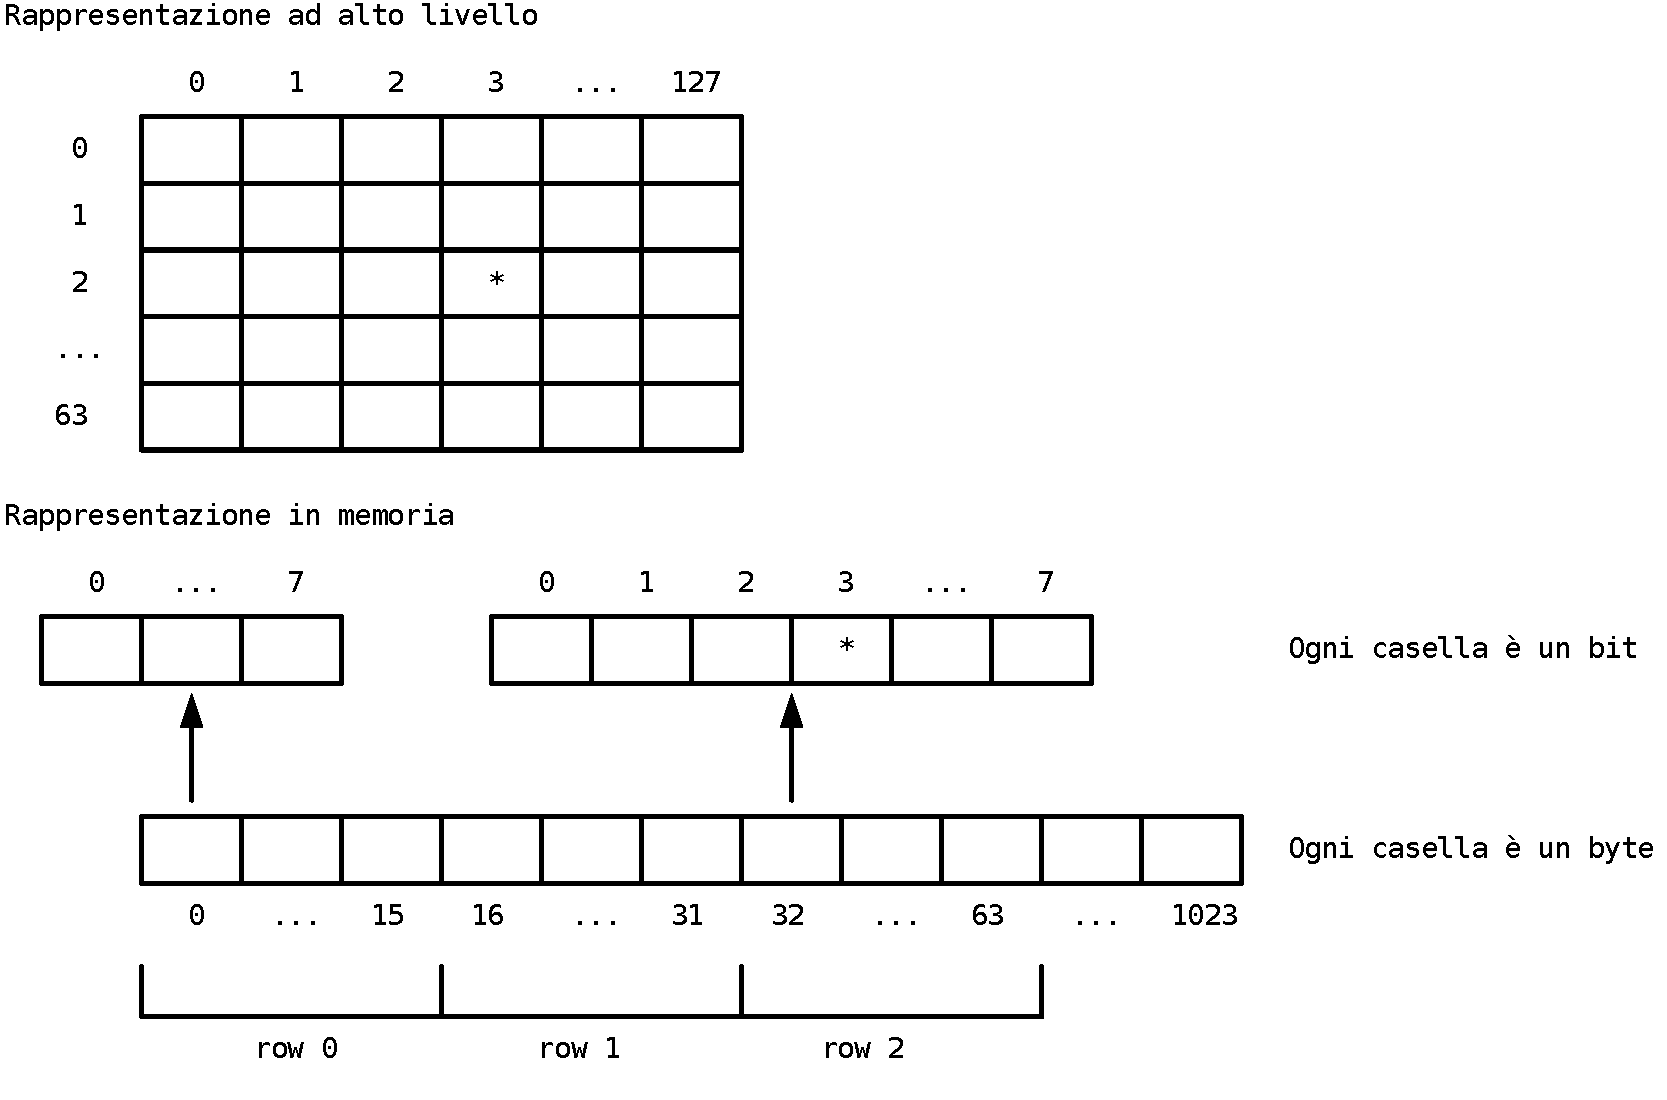
\includegraphics[scale=0.50]{figures/screenopt.pdf}
    \end{center}
    \caption{Esempio della mappatura di un pixel.}
    \label{fig:screenopt}
\end{figure}

% TODO: Update dello schermo solo se è cambiato lo schermo

È stato necessario introdurre delle ottimizzazioni all'interno
dell'interprete per poterlo far girare su un microcontrollore.

L'ottimizzazione principale è legata alla rappresentazione
dello schermo in memoria. Ad alto livello lo schermo può essere
visto come una matrice di 128x64 pixel monocromi. Purtroppo però
una rappresentazione simile, dove ciascun pixel viene rappresentato
da un byte occuperebbe 8192 byte, e dobbiamo considerare il fatto
che il nostro microcontrollore ha a disposizione solamente di 16 Kb
di SRAM.

Per questo motivo abbiamo deciso di rappresentare lo schermo come
un array unidimensionale di 1024 byte, dove ciascun pixel viene
rappresentato con un singolo bit. Questa decisione ha aggiunto però
un livello di indirezione dato che una coordinata ad alto livello
sulla matrice 128x64 deve essere mappata ad una coordinata
"in memoria".

\subsubsection{Quirks}

% TODO

% Le piattaforme supportate dall'interprete sono CHIP-8, CHIP-48,
% S-CHIP 1.0 e S-CHIP 1.1.

\subsection{Architettura}

% TODO: aggiornare il class diagram e il sequence diagram

% \section{Assemblaggio}

% TODO

\section{Analisi del consumo energetico} % ALT: Alimentazione e consumi

% TODO

\section{Considerazioni finali} % ALT: Conclusioni e sviluppi futuri

% TODO

\addcontentsline{toc}{section}{Riferimenti bibliografici}
\bibliographystyle{plain}
\bibliography{report}

\end{document}
